%cc/cv de overleaf.com :s
\documentclass{beamer}
\usetheme{Frankfurt}
\usecolortheme{seahorse}
\title{Super titre de TIPE}
\subtitle{sous-titre}
\author{Alexandrine, Pedro\\\and De Carvalho, Enzo}
\date{2020-2021}

\usepackage{xurl}
\usepackage{graphicx}
\graphicspath{ {figures/} }

\begin{document}

\begin{frame}
	\maketitle
\end{frame}

\begin{frame}
	\frametitle{Sommaire}
	\tableofcontents
\end{frame}

\section{Première approche : simple regression}
\subsection{Regression linéaire (ElasticNet)}
\begin{frame}
	\frametitle{Regression linéaire}
	ElasticNet ne fait que des droites, c'est pas intéressant.
	\begin{figure}[b]
		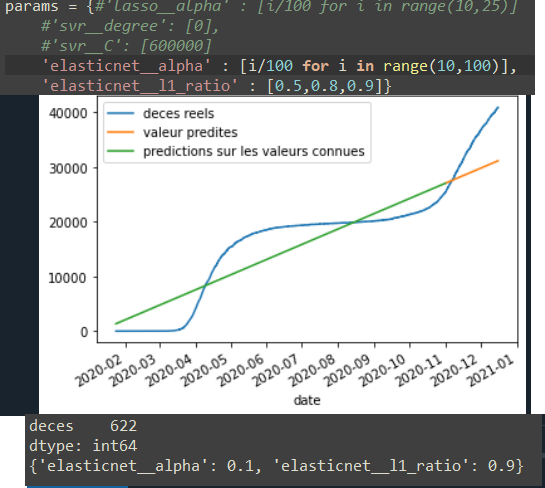
\includegraphics[scale=0.4]{EN}
		\centering
	\end{figure}
\end{frame}

\subsection{Optimisation d'hyperparamètres et stratégies}
\begin{frame}
	\frametitle{Hyperparamètre}
	là on explique en quoi consiste l'optimisation d'hyperparamètres (crossvalidation)
	Et pourquoi on est passer du découpage de base que propose GridSearchCV (k-fold) au découpage tscv (time-split series)
	\\
	\alert{lien utile : }
	\url{https://scikit-learn.org/stable/auto_examples/model_selection/plot_cv_indices.html########sphx-glr-auto-examples-model-selection-plot-cv-indices-py}
\end{frame}

\subsection{Résultats avec SVR}
\begin{frame}
	\frametitle{SVR ; premier résultat}
	Approche à l'aide du modèle SVR (avec le noyau 'rbf') (Support Vector Regressor)
	\begin{figure}[tc]
		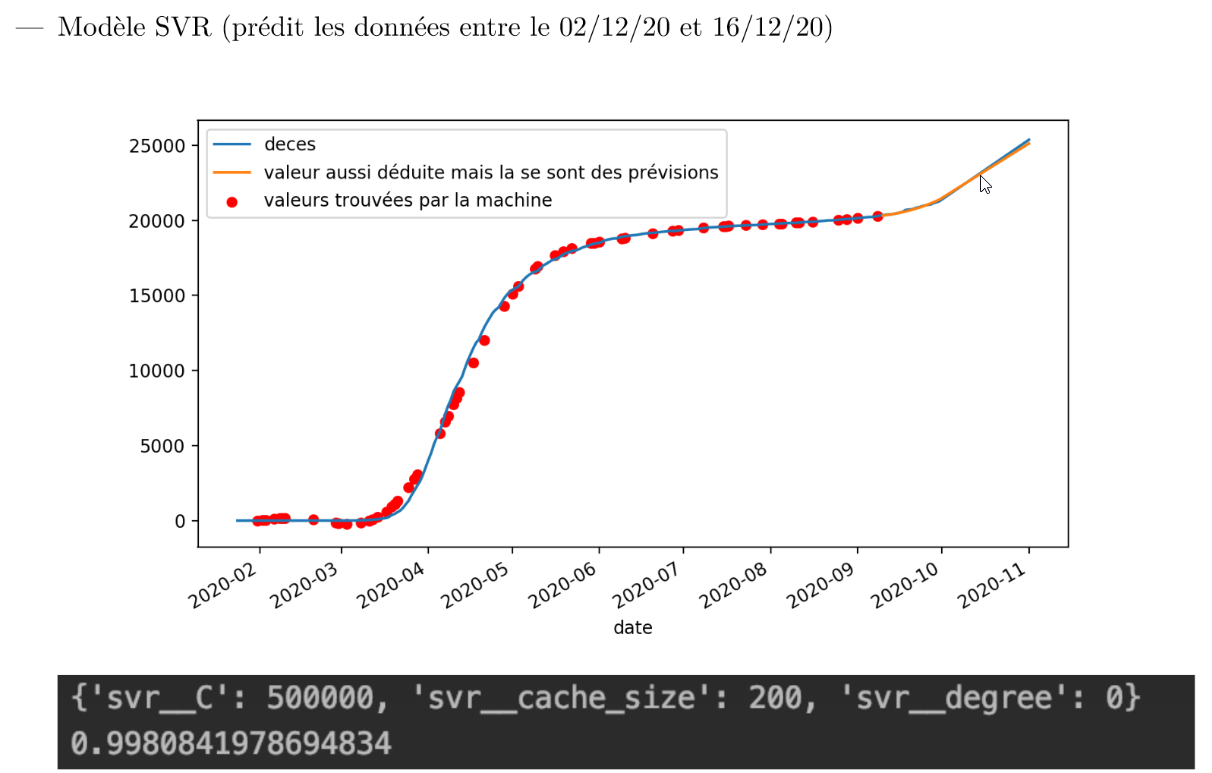
\includegraphics[scale=0.2]{SVR_premierdecoup}
		\centering
		\caption{Premier résultat avec SVR (avec une "mauvaise stratégie" de découpage pour former un modèle prédisant une série temporelle}
	\end{figure}
\end{frame}
\begin{frame}
	\frametitle{SVR}
	\begin{figure}[t]
		\centering
		\begin{minipage}{0.5\textwidth}
			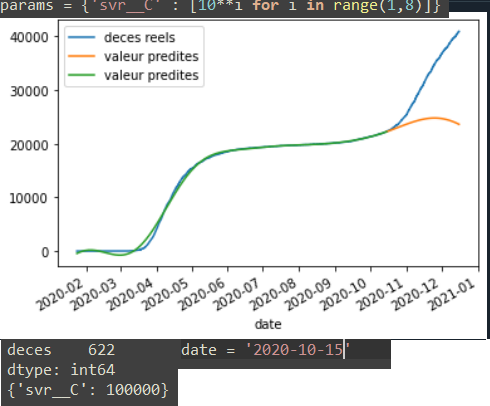
\includegraphics[scale=0.25]{SVR_avant_pt_dinflexion}
		\end{minipage}%
		\begin{minipage}{0.5\textwidth}
			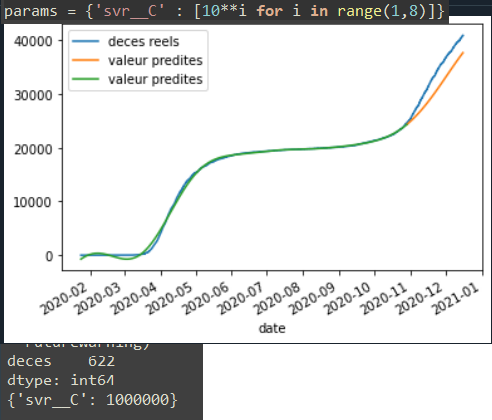
\includegraphics[scale=0.25]{SVR_apres_pt_dinflexion}
		\end{minipage}
	\caption{à gauche la prediction avant le pt d'inflexion, à droite, après.}
	\end{figure}
\end{frame}
\begin{frame}
	\frametitle{fbprophet}
	Approche avec le module fbprophet (designé pour prédire des séries temporelles)
	\begin{figure}[t]
		\begin{minipage}{0.3\textwidth}
			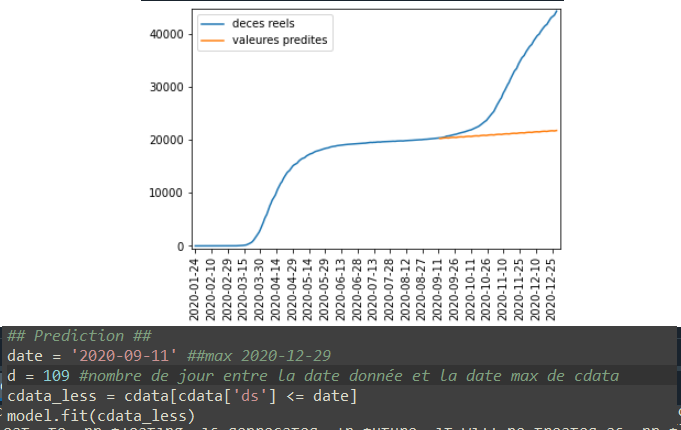
\includegraphics[scale=0.13]{fbprophet_avant_pt_dinflexion}
		\end{minipage}
		\begin{minipage}{0.3\textwidth}
			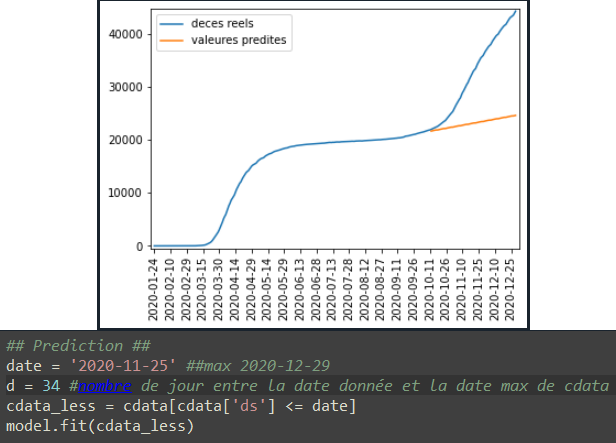
\includegraphics[scale=0.13]{fbprophet_mid_pt_dinflexion}
		\end{minipage}
		\begin{minipage}{0.3\textwidth}
			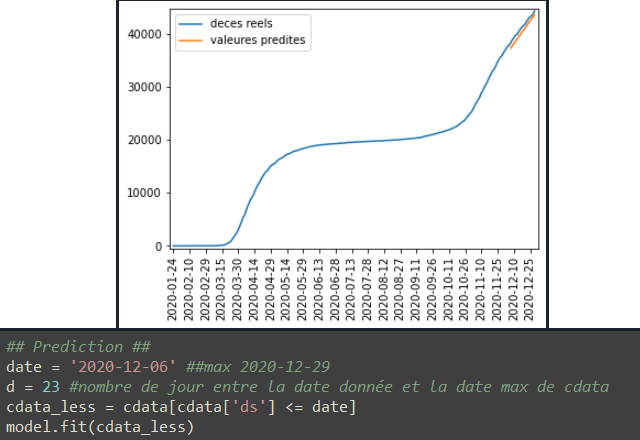
\includegraphics[scale=0.13]{fbprophet_apres_pt_dinflexion}
		\end{minipage}
	\caption{résultats avec fbprophet (insatisfaisant)}
	\end{figure}
\end{frame}

\section{Approche multivariées}
\subsection{Multiregresseur : 'RegressorChain'}
\begin{frame}
	\frametitle{RegressorChain SVR}
	Approche avec le multiregresseur\\
	\tiny{(description de scikit : \url{https://scikit-learn.org/stable/modules/generated/sklearn.multioutput.RegressorChain.html########sklearn.multioutput.RegressorChain})}\\
	\normalsize{\textit{"Each model makes a prediction in the order specified by the chain using all of the available features provided to the model plus the predictions of models that are earlier in the chain."}}
	\begin{figure}[h]
		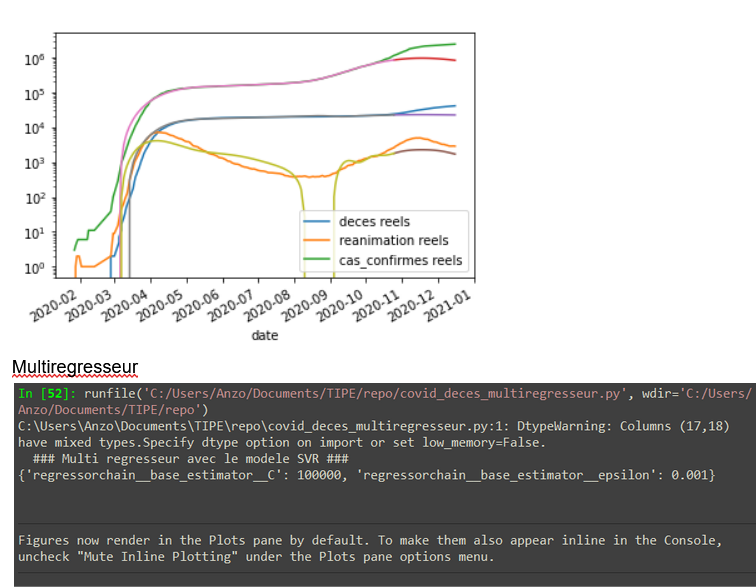
\includegraphics[scale=0.3]{mulitregr_epic_fail}
		\caption{bug qu'on a pas reussi à corriger sous ces conditions}
	\end{figure}
\end{frame}

\subsection{Réseau neuronal}
\begin{frame}
	\frametitle{Explications}
	Là on explique savamment l'art du réseau neuronal
\end{frame}

\begin{frame}
	\frametitle{Résultats}
	\begin{figure}[h]
		\centering
		\begin{minipage}{0.5\textwidth}
			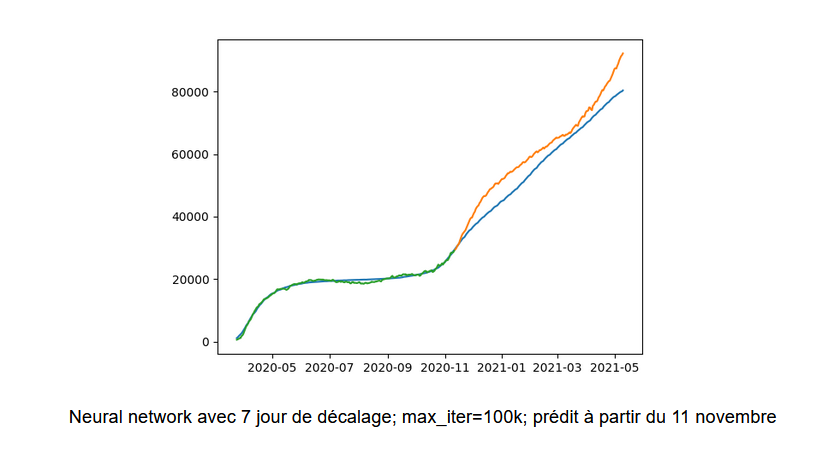
\includegraphics[width=\textwidth]{NN_1}
			\centering
		\end{minipage}
		\begin{minipage}{0.5\textwidth}
			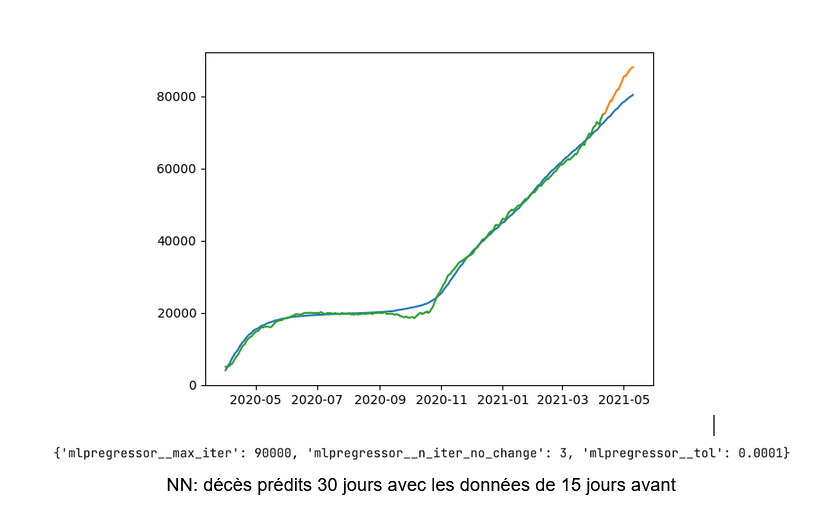
\includegraphics[width=\textwidth]{NN_2}
			\centering
		\end{minipage}
	\end{figure}
\end{frame}

\begin{frame}
	\frametitle{Résultats}
	\begin{figure}
		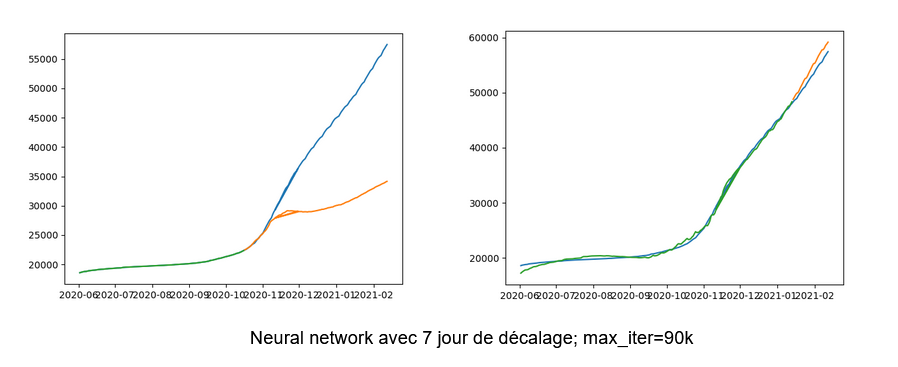
\includegraphics[scale=0.6]{NN_3}
		\caption{échec du modèle sans la courbe des cas confirmés}
	\end{figure}
\end{frame}

\end{document}
